% Filename: lista10.tex
% 
% This code is part of 'Solutions for MT402, Matrizes'
% 
% Description: This file corresponds to the solutions of homework sheet 10.
% 
% Created: 24.04.12 05:54:57 PM
% Last Change: 04.06.12 05:12:27 PM
% 
% Authors:
% - Raniere Silva (2012): initial version
% 
% Copyright (c) 2012 Raniere Silva <r.gaia.cs@gmail.com>
% 
% This work is licensed under the Creative Commons Attribution-ShareAlike 3.0 Unported License. To view a copy of this license, visit http://creativecommons.org/licenses/by-sa/3.0/ or send a letter to Creative Commons, 444 Castro Street, Suite 900, Mountain View, California, 94041, USA.
%
% This work is distributed in the hope that it will be useful, but WITHOUT ANY WARRANTY; without even the implied warranty of MERCHANTABILITY or FITNESS FOR A PARTICULAR PURPOSE.
%
\begin{questions}
    \question Considere $A : m \times n$, $m \geq n$ e $\bar{x} \in \mathbb{R}^n$. Demonstre que: $\| b - A \bar{x} \|_2 = \min_{y \in \mathbb{R}^n} \| b - A y \|_2$ se e somente se $(b - A \bar{x}) \in \text{Im}(A)^\perp$.
    \begin{solution}
        Na p\'{a}gina 438 do Meyer\nocite{Meyer:2000:matrix}, temos que o problema de m\'{i}nimos quadrados consiste em encontrar $x$ tal que $A x = P_{\text{Im}(A)} b$. Mas este sistema \'{e} tal que
        \begin{align*}
            A x = P_{\text{Im}(A)} b &\leftrightarrow P_{\text{Im}(R)} A x = P_{\text{Im}(A)} P_{\text{Im}(A)} b = P_{\text{Im}(A)} b \\
            &\leftrightarrow P_{\text{Im}(A)} \left( A x - b \right) = 0 \\
            &\leftrightarrow \left( A x - b \right) \in \text{N}(P_{\text{Im}(A)}) = \text{Im}(A)^\perp = \text{N}(A^t).
        \end{align*}
    \end{solution}

    \question Seja $\bar{x} \in \mathbb{R}^n$. Ent\~{a}o, $\bar{x}$ resolve o problema de quadrados m\'{i}nimos para $A x = b$, se e somente se $A^t A \bar{x} = A^t b$.
    \begin{solution}
        Se $\bar{x}$ \'{e} a solu\c{c}\~{a}o do problema de quadrados m\'{i}nimos de $A x = b$ ent\~{a}o
        \begin{align*}
            \bar{x} \mid \| A \bar{x} - b \| = \min \| A x - b \| &\leftrightarrow Q^t A \bar{x} = Q^t b \\
            &\leftrightarrow R \bar{x} = Q^t b \\
            &\leftrightarrow R^t R \bar{x} = R^t Q^t b \\
            &\leftrightarrow R^t Q^t Q R \bar{x} = R^t Q^t b \\
            &\leftrightarrow A^t A \bar{x} = A^t b.
        \end{align*}
    \end{solution}

    \question Considere $A : m \times n$, $m \geq n$ e sua fatora\c{c}\~{a}o ortogonal dada por $A = Q R$ com $Q : m \times m$ ortogonal e $R : m \times n$, com coeficientes $r_{ij} = 0$, $i > j$. Reescreva a solu\c{c}\~{a}o de quadrados m\'{i}nimos $\bar{x} = \left( A^t A \right)^{-1} A^t b$ e a proje\c{c}\~{a}o ortogonal de $b \in \text{Im}(A)$ usando a fatora\c{c}\~{a}o ortogonal de $A$. Relacione as express\~{o}es obtidas com a solu\c{c}\~{a}o de quadrados m\'{i}nimos obtida diretamente da fatora\c{c}\~{a}o ortogonal: $\| b - A x \|_2 = \| Q^t \left( b - A x \right) \|_2$ \ldots
    \begin{solution}
        Podemos reescrever a solu\c{c}\~{a}o da seguinte forma:
        \begin{align*}
            \bar{x} &= \left( A^t A \right)^{-1} A^t b \\
            &= \left( R^t Q^t Q R \right)^{-1} R^t Q^t b \\
            &= \left( R^t R \right)^{-1} R^t Q^t b \\
            &= R^{-1} R^{-t} R^t Q^t b \\
            &= R^{-1} Q^t b.
        \end{align*}

        E a proje\c{c}\~{a}o ortogonal de $b \in \text{Im}(A)$ corresponde a
        \begin{align*}
            P_{\text{Im}(A)} b &= (I - Q) b.
        \end{align*}
    \end{solution}

    \question Considere
    \begin{align*}
        A = \begin{bmatrix}
            1 & 2 \\
            0 & 1 \\
            1 & 0
        \end{bmatrix}.
    \end{align*}
    \begin{parts}
        \part Construa o projetor ortogonal $P$ sobre o subespa\c{c}o $\text{Im}(A)$. Obtenha a proje\c{c}\~{a}o do vetor $v = \left( 1, -1, 2 \right)^t$ em $\text{Im}(A)$. Idem para o vetor $w = \left( 1, 1, -1 \right)^t$.
        \begin{solution}
            Na p\'{a}gina 430 do Meyer\nocite{Meyer:2000:matrix}, temos:
            \begin{quote}
                Seja $\mathcal{M}$ um subespa\c{c}o $r$-dimensional de $\mathbb{R}$, e seja as colunas de $M_{n \times r}$ e $N_{n \times {n - r}}$ as bases de $\mathcal{M}$ e $\mathcal{M}^\perp$, respectivamente. Ent\~{a}o os projetores ortogonais de $\mathcal{M}$ e $\mathcal{M}^\perp$ s\~{a}o
                \begin{align*}
                    P_{\mathcal{M}} &= M \left( M^t M \right)^{-1} M^t \text{ e } P_{\mathcal{M}^\perp} = N \left( N^t N \right)^{-1} N^t.
                \end{align*}
                Se $M$ e $N$ s\~{a}o bases ortonormais para $\mathcal{M}$ e $\mathcal{M}^\perp$, ent\~{a}o
                \begin{align*}
                    P_{\mathcal{M}} &= M M^t \text{ e } P_{\mathcal{M}^\perp} = N N^t.
                \end{align*}
            \end{quote}

            Ent\~{a}o,
            \begin{align*}
                P &= A A^t = \begin{bmatrix}
                    5 & 2 & 1 \\
                    2 & 1 & 0 \\
                    1 & 0 & 1
                \end{bmatrix}.
            \end{align*}
            E portanto,
            \begin{align*}
                P v &= \begin{bmatrix}
                    5 & 2 & 1 \\
                    2 & 1 & 0 \\
                    1 & 0 & 1
                \end{bmatrix} \begin{bmatrix}
                    1 \\
                    -1 \\
                    2
                \end{bmatrix} = \begin{bmatrix}
                    5 \\
                    1 \\
                    3
                \end{bmatrix},
                P w &= \begin{bmatrix}
                    5 & 2 & 1 \\
                    2 & 1 & 0 \\
                    1 & 0 & 1
                \end{bmatrix} \begin{bmatrix}
                    1 \\
                    1 \\
                    -1
                \end{bmatrix} = \begin{bmatrix}
                    6 \\
                    3 \\
                    0
                \end{bmatrix}
            \end{align*}

            Geometricamente temos
            \begin{center}
                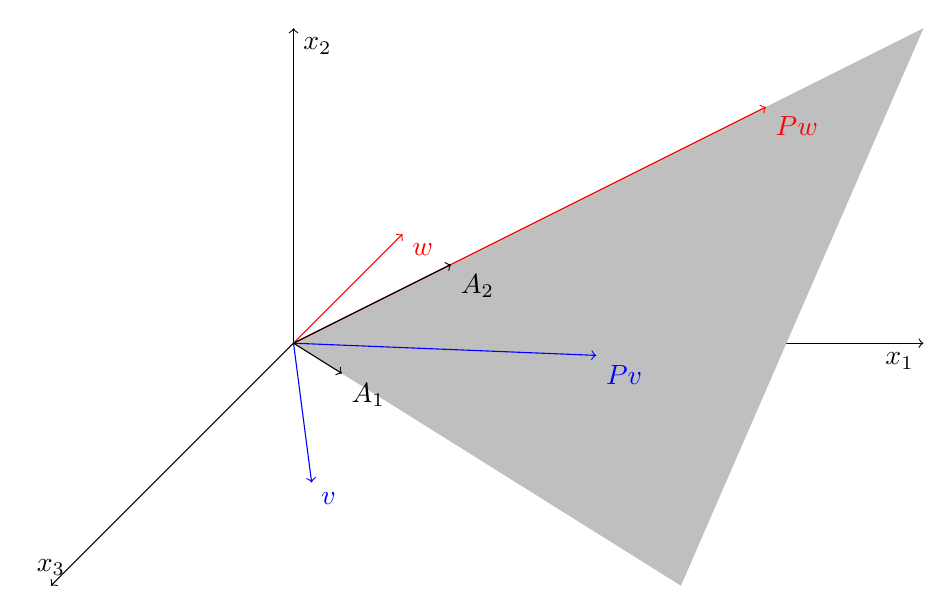
\begin{tikzpicture}
                    \coordinate (O) at (0,0,0);
                    \draw[->] (0,0,0) -- (8,0,0) node[anchor=north east]{$x_1$};
                    \draw[->] (0,0,0) -- (0,4,0) node[anchor=north west]{$x_2$};
                    \draw[->] (0,0,0) -- (0,0,8) node[anchor=south]{$x_3$};

                    \fill[color=gray!50] (0, 0, 0) -- (8, 0, 8) -- (8, 4, 0) -- (0, 0, 0);

                    \draw[->, color=blue] (0, 0, 0) -- (1, -1, 2) node[below right] {$v$};
                    \draw[->, color=blue] (0, 0, 0) -- (5, 1, 3) node[below right] {$P v$};

                    \draw[->, color=red] (0, 0, 0) -- (1, 1, -1) node[below right] {$w$};
                    \draw[->, color=red] (0, 0, 0) -- (6, 3, 0) node[below right] {$P w$};

                    \draw[->] (0, 0, 0) -- (1, 0, 1) node[below right] {$A_{\mdot 1}$};
                    \draw[->] (0, 0, 0) -- (2, 1, 0) node[below right] {$A_{\mdot 2}$};
                \end{tikzpicture}
            \end{center}
        \end{solution}

        \part Obtenha a fatora\c{c}\~{a}o QR reduzida de $A$.
        \begin{solution}
            Para obter a fatora\c{c}\~{a}o QR reduzida podemos utilizar o M\'{e}todo de Gram-Schmidt Modificado.

            O algoritmo a seguir, retirado do Golub\nocite{Golub:1996:matrix} (p\'{a}gina 231), tem como entrada $A \in \mathbb{R}^{m \times n}$ de posto completo e calcula a fatora\c{c}\~{a}o QR reduzida de $A$ onde $Q \in \mathbb{R}^{m \times n}$ tem colunas ortonormais e $R \in \mathbb{R}^{n \times n}$ \'{e} triangular superior.
            \begin{algorithmic}
                \For{$k = 1, \ldots, n$}
                    \State $R(k, k) \leftarrow \| A(1:m, k) \|_2$
                    \State $Q(1:m, k) \leftarrow A(1:m, k) / R(k,k)$
                    \For{$j = k + 1 : n$}
                        \State $R(k, j) \leftarrow Q(1:m, k)^t A(1:m, j)$
                        \State $A(1:m, j) \leftarrow A(1:m, j) - Q(1:m, k) R(k, j)$
                    \EndFor
                \EndFor
            \end{algorithmic}

            Aplicando ao algoritmo acima, temos
            \begin{enumerate}
                \item $k = 1$:
                    \begin{align*}
                        R &\leftarrow \begin{bmatrix}
                            \sqrt{2} & \left( 1 / \sqrt{2} \right) 2 + 0 \left( 1 \right) + \left( 1 / \sqrt{2} \right) 0 \\
                            0 & 0
                        \end{bmatrix} = \begin{bmatrix}
                            \sqrt{2} & 2 / \sqrt{2} \\
                            0 & 0
                        \end{bmatrix}, \\
                        Q &\leftarrow \begin{bmatrix}
                            1 / \sqrt{2} & 0 \\
                            0 & 0 \\
                            1 / \sqrt{2} & 0
                        \end{bmatrix}, \\
                        A &\leftarrow \begin{bmatrix}
                            1 & 2 - \left( 1 / \sqrt{2} \right) \left( 2 / \sqrt{2} \right) \\
                            0 & 1 - 0 \left( 2 / \sqrt{2} \right) \\
                            1 & 0 - \left( 1 / \sqrt{2} \right) \left( 2 / \sqrt{2} \right)
                        \end{bmatrix} = \begin{bmatrix}
                            1 & 1 \\
                            0 & 1 \\
                            1 & -1
                        \end{bmatrix}.
                    \end{align*}

                \item $k = 2$:
                    \begin{align*}
                        R &\leftarrow \begin{bmatrix}
                            \sqrt{2} & 2 / \sqrt{2} \\
                            0 & \sqrt{3}
                        \end{bmatrix}, \\
                        Q &\leftarrow \begin{bmatrix}
                            1 / \sqrt{2} & 1 / \sqrt{3} \\
                            0 & 1 / \sqrt{3} \\
                            1 / \sqrt{2} & -1 / \sqrt{3}
                        \end{bmatrix}, \\
                        A &\leftarrow \begin{bmatrix}
                            1 & 1 \\
                            0 & 1 \\
                            1 & -1
                        \end{bmatrix}.
                    \end{align*}
            \end{enumerate}
        \end{solution}

        \part Obtenha a fatora\c{c}\~{a}o QR de $A$ atrav\'{e}s dos m\'{e}todos de Householder e Givens.
        \begin{solution}
            Primeiro vamos obter a fatora\c{c}\~{a}o QR atrav\'{e}es do m\'{e}todo de Householder.

            O algoritmo a seguir, retirado do Golub\nocite{Golub:1996:matrix} (p\'{a}gina 224), tem como entrada $A \in \mathbb{R}^{m \times n}$ com $m \geq n$ e encontra as matrizes de Householder $H_1, \ldots, H_n$ tal que se $Q = H_1 \ldots H_n$ ent\~{a}o $Q^t A = R$ que \'{e} triangular superior. A parte triangular superior da matriz $A$ \'{e} sobrescrita pela parte triangular superior de $R$ e as componentes $j + 1 : n$ do $j$-\'{e}simo vetor de Householder \'{e} armazenado em $A(j + 1:m, j)$, $j < m$.
            \begin{algorithmic}
                \For{$j = 1, \ldots, n$}
                    \State $[v, \beta] \leftarrow \text{\bf householder}(A(j:m, j))$
                    \State $A(j:m, j:n) \leftarrow \left( I_{m - j + 1} - \beta v v^t \right) A(j:m, j:n)$
                    \If{$j < m$}
                        \State $A(j + 1:m, j) \leftarrow v(2:m - j + 1)$
                    \EndIf
                \EndFor
            \end{algorithmic}

            Aplicando uma vers\~{a}o modificada do algoritmo acima, temos
            \begin{enumerate}
                \item $j = 1$:
                    \begin{align*}
                        x &\leftarrow \begin{bmatrix}
                            1 \\
                            0 \\
                            1
                        \end{bmatrix}, v \leftarrow \begin{bmatrix}
                            1 + \sqrt{2} \\
                            0 \\
                            1
                        \end{bmatrix} \approx \begin{bmatrix}
                            2.41 \\
                            0 \\
                            1
                        \end{bmatrix}\\
                        A &\leftarrow A - (2 / v^t v) v (v^t A) = \begin{bmatrix}
                            1 & 2 \\
                            0 & 1 \\
                            1 & 0
                        \end{bmatrix} -  (1 / 3.41) \begin{bmatrix}
                            8.23 & 11.64 \\
                            0.00 & 0.00 \\
                            3.41 & 4.82
                        \end{bmatrix} \\
                        &\quad = \begin{bmatrix}
                            1 & 2 \\
                            0 & 1 \\
                            1 & 0
                        \end{bmatrix} -  \begin{bmatrix}
                            2.41 & 3.41 \\
                            0.00 & 0.00 \\
                            1.00 & 1.41
                        \end{bmatrix}  = \begin{bmatrix}
                            -1.41 & - 1.41 \\
                            0 & 1 \\
                            0 & - 1.41
                        \end{bmatrix}
                    \end{align*}

                \item $j = 2$:
                    \begin{align*}
                        x &\leftarrow \begin{bmatrix}
                            1 \\
                            -1.41
                        \end{bmatrix}, v \leftarrow \begin{bmatrix}
                            2.72 \\
                            -1.41
                        \end{bmatrix} \\
                        A(2:3, 2:2) &\leftarrow A(2:3, 2:2) - (2 / v^t v) v (v^t A(2:3, 2:2) \\
                        &\quad = \begin{bmatrix}
                            1 \\
                            -1.41
                        \end{bmatrix} - \begin{bmatrix}
                            2.72 \\
                            -1.41
                        \end{bmatrix} = \begin{bmatrix}
                            -1.72 \\
                            0
                        \end{bmatrix}, \\
                        A &\leftarrow \begin{bmatrix}
                            -1.41 & -1.41 \\
                            0 & -1.72 \\
                            0 & 0
                        \end{bmatrix}.
                    \end{align*}
            \end{enumerate}

            Agora vamos obter a fatora\c{c}\~{a}o QR atrav\'{e}es do m\'{e}todo de Givens.

            O algoritmo a seguir, retirado do Golub\nocite{Golub:1996:matrix} (p\'{a}gina 227), tem como entrada $A \in \mathbb{R}^{m \times n}$ com $m \geq n$ e sobrescreve a matriz $A$ tal que $Q^t A = R$, onde $R$ \'{e} triangular superior e $Q$ \'{e} ortogonal.
            \begin{algorithmic}
                \For{$j = 1, \ldots, n$}
                    \For{$i = m : - 1 : j + 1$}
                        \State $[c, s] \leftarrow \text{\bf givens}(A(i - 1, j), A(i, j))$
                        \State $A(i - 1:i, j:n) \leftarrow \begin{bmatrix}
                            c & s \\
                            -s & c
                        \end{bmatrix}^t A(i - 1:i, j:n)$
                    \EndFor
                \EndFor
            \end{algorithmic}

            Aplicando uma vers\~{a}o modificada do algoritmo acima com detec\c{c}\~{a}o de zero, temos
            \begin{enumerate}
                \item $i = 1$, $k = 3$ e $j = 1$:

                    $c = 1 / \sqrt{2}$ e $s = 1 / \sqrt{2}$. Portanto
                    \begin{align*}
                        A &\leftarrow \begin{bmatrix}
                            2 / \sqrt{2} & 2 / \sqrt{2} \\
                            0 & 1 \\
                            0 & - 2 / \sqrt{2}
                        \end{bmatrix}.
                    \end{align*}
                    
                \item $i = 1$, $k = 2$ e $j = 1$:

                    N\~{a}o precisa ser feito nada, pois $a_{21} = 0$.

                \item $i = 2$, $k = 3$ e $j = 2$:

                    $c = 1 / \sqrt{2}$ e $s = -2 / \sqrt{6}$. Portanto
                    \begin{align*}
                        A &\leftarrow \begin{bmatrix}
                            2 / \sqrt{2} & 2 / \sqrt{2} \\
                            0 & 3 / \sqrt{3} \\
                            0 & 0
                        \end{bmatrix}.
                    \end{align*}
            \end{enumerate}
        \end{solution}

        \part Obtenha a solu\c{c}\~{a}o de Quadrados M\'{i}nimos para $A x = v$, atrav\'{e}s da resolu\c{c}\~{a}o do sistema linear com equa\c{c}\~{o}es normais e atrav\'{e}s do processo de fatora\c{c}\~{o}es ortogonais.
        \begin{solution}
            Primeiro vamos resolver o sistema utilizando equa\c{c}\~{o}es normais, i.e., $A^t A x = A^t v$. Ent\~{a}o,
            \begin{align*}
                \begin{bmatrix}
                    1 & 0 & 1 \\
                    2 & 1 & 0
                \end{bmatrix} \begin{bmatrix}
                    1 & 2 \\
                    0 & 1 \\
                    1 & 0
                \end{bmatrix} x &= \begin{bmatrix}
                    1 & 0 & 1 \\
                    2 & 1 & 0
                \end{bmatrix} \begin{bmatrix}
                    1 \\
                    -1 \\
                    2
                \end{bmatrix} \\
                \begin{bmatrix}
                    2 & 2 \\
                    2 & 5
                \end{bmatrix} x &= \begin{bmatrix}
                    3 \\
                    1
                \end{bmatrix} \\
                \begin{bmatrix}
                    2 & 2 \\
                    0 & 3
                \end{bmatrix} x &= \begin{bmatrix}
                    3 \\
                    -1
                \end{bmatrix}.
            \end{align*}
            Portanto, $x_1 = 13/ 6$ e $x_2 = -2 / 3$.

            Agora vamos resolver o problema com fatora\c{c}\~{o}es ortogonais (utilizando Givens).

            Antes de resolvermos o sistema triangular, precisamos adequar o lado direito.
            \begin{align*}
                \begin{bmatrix}
                    1 & 0 & 0 \\
                    0 & 1 / \sqrt{3} & -2 / \sqrt{6} \\
                    0 & 2 / \sqrt{6} & 1 / \sqrt{3}
                \end{bmatrix} \begin{bmatrix}
                    1 / \sqrt{2} & 0 & 1 / \sqrt{2} \\
                    0 & 1 & 0 \\
                    - 1 / \sqrt{2} & 0 & 1 \sqrt{2}
                \end{bmatrix} \begin{bmatrix}
                    1 \\
                    -1 \\
                    2
                \end{bmatrix} &= \begin{bmatrix}
                    1 & 0 & 0 \\
                    0 & 1 / \sqrt{3} & -2 / \sqrt{6} \\
                    0 & 2 / \sqrt{6} & 1 / \sqrt{3}
                \end{bmatrix} \begin{bmatrix}
                    3 / \sqrt{2}  \\
                    -1 \\
                    1 / \sqrt{2}
                \end{bmatrix} \\
                &= \begin{bmatrix}
                    3 / \sqrt{2}  \\
                    -2 / \sqrt{3} \\
                    - 1 / \sqrt{6}
                \end{bmatrix} 
            \end{align*}
            Ent\~{a}o temos seguinte sistema triangular
            \begin{align*}
                \begin{bmatrix}
                    2 / \sqrt{2} & 2 / \sqrt{2} \\
                    0 & 3 / \sqrt{3}
                \end{bmatrix} x &= \begin{bmatrix}
                    3 / \sqrt{2} \\
                    -2 / \sqrt{3}
                \end{bmatrix}
            \end{align*}
            cuja solu\c{c}\~{a}o \'{e} $x_1 = 13 / 6$ e $x_2 = -2 / 3$.
        \end{solution}
    \end{parts}

    \question Seja o sistema linear $A x = b$, $A : m \times n$, $m > n$, $\text{posto}(A) = r$. Fa\c{c}a um resumo sobre a solu\c{c}\~{a}o de Quadrados M\'{i}nimos deste sistema. Analise a exist\^{e}ncia e unicidade desta solu\c{c}\~{a}o usando as equa\c{c}\~{o}es normais e as fatora\c{c}\~{o}es ortogonais. Considere os casos $r = n$ e $r < n$ e inclua em sua an\'{a}lise o caso em que $b \in \text{Im}(A)$.
    \begin{solution}
        A solu\c{c}\~{a}o de Quadrados M\'{i}nimos \'{e} representada na tabela abaixo.
        \begin{center}
            \begin{tabular}{|p{.15\textwidth}|p{.15\textwidth}|p{.15\textwidth}|p{.15\textwidth}|p{.15\textwidth}|}
                \cline{2-5}
                \multicolumn{1}{c|}{} & \multicolumn{2}{|c|}{$r = n$} & \multicolumn{2}{|c|}{$r < n$} \\ \cline{2-5}
                \multicolumn{1}{c|}{} & $b \in \text{Im}(A)$ & $b \not\in \text{Im}(A)$ & $b \in \text{Im}(A)$ & $b \not\in \text{Im}(A)$ \\ \hline
                Quadrados M\'{i}nimos & Solu\c{c}\~{a}o \'{u}nica com res\'{i}duo igual de zero & Solu\c{c}\~{a}o \'{u}nica com res\'{i}duo diferente de zero & Infinitas solu\c{c}\~{o}es com res\'{i}duo igual a zero & Infinitas solu\c{c}\~{o}es com res\'{i}duo diferente de zero \\ \hline
                Equa\c{c}\~{o}es Normais & Solu\c{c}\~{a}o \'{u}nica & Solu\c{c}\~{a}o \'{u}nica & $A^t A$ \'{e} singular & $A^t A$ \'{e} singular \\ \hline
                Fatora\c{c}\~{o}es Ortogonais & Solu\c{c}\~{a}o \'{u}nica & Solu\c{c}\~{a}o \'{u}nica & $R$ \'{e} trapezoidal & $R$ \'{e} trapezoidal \\ \hline
            \end{tabular}
        \end{center}
    \end{solution}

    \question Sistema Linear Aumentado: Considere $A : m \times n$, $m > n$, $\text{posto}(A) = n$ e o sistema linear $A x = b$. O sistema linear aumentado \'{e} dado por $B y = c$, onde
    \begin{align*}
        B &= \begin{bmatrix}
            I & A \\
            A^t & 0
        \end{bmatrix}, & y &= \begin{bmatrix}
            r \\
            x
        \end{bmatrix}, & c &= \begin{bmatrix}
            b \\
            0
        \end{bmatrix},
    \end{align*}
    onde $I : m \times m$ \'{e} a matriz identidade.

    Este sistema linear admite solu\c{c}\~{a}o \'{u}nica (por qu\^{e}?). Relacione a solu\c{c}\~{a}o deste sistema linear dada pelos vetores: $r^*$ e $x^*$ com a solu\c{c}\~{a}o de problema de Quadrados M\'{i}nimos para $A x = b$. Quais m\'{e}todos podem ser aplicados para resolver $B y = c$?
    \begin{solution}
        Considerando o sistema linear
        \begin{align*}
            \begin{bmatrix}
                I & A \\
                A^t & 0
            \end{bmatrix} \begin{bmatrix}
                r \\
                x
            \end{bmatrix} &= \begin{bmatrix}
                b \\
                0
            \end{bmatrix}
        \end{align*}
        temos que $A^t r = 0$ e $I r + A x = b$. Portanto $r = b - A x$ e substituindo na outra equa\c{c}\~{a}o obtemos
        \begin{align*}
            A^t \left( b - A x \right) &= 0 \leftrightarrow A^t A x = A^tb
        \end{align*}
        que corresponde ao sistema normal. Como $A$ tem posto completo sabemos que o sistema de equa\c{c}\~{o}es normais possue solu\c{c}\~{a}o \'{u}nica.
    \end{solution}

    \question Considere o sistema linear $A x = b$, $A : m \times n$, $m > n$ e a solu\c{c}\~{a}o de Quadrados M\'{i}nimos para este sistema, $\bar{x}$. Se multiplicarmos a equa\c{c}\~{a}o $j$ por $\alpha \neq 0$, obtemos assim o sistema $B x = d$, a solu\c{c}\~{a}o de Quadrados M\'{i}nimos permanece a mesma? Justifique.
    \begin{solution}
        A solu\c{c}\~{a}o do sistema $B x = d$ pode ser diferente da solu\c{c}\~{a}o do sistema $A x = b$. Esse fato pode ser observado ao comparar os sistemas de equa\c{c}\~{o}es normais de cada um dos sistemas pois
        \begin{align*}
            A &= \begin{bmatrix}
                A_{1 \mdot} \\
                A_{2 \mdot} \\
                \vdots \\
                A_{m \mdot}
            \end{bmatrix}, \\
            A^t A &= \begin{bmatrix}
                A_{1 \mdot}^t & A_{2 \mdot}^t & \ldots & A_{m \mdot}^t
            \end{bmatrix} \begin{bmatrix}
                A_{1 \mdot} \\
                A_{2 \mdot} \\
                \vdots \\
                A_{m \mdot}
            \end{bmatrix} \\
            &= A_{1 \mdot}^t A_{1 \mdot} + A_{2 \mdot}^t A_{2 \mdot} + \ldots + A_{m \mdot}^t A_{m \mdot}, \\
            B &= \begin{bmatrix}
                \alpha A_{1 \mdot} \\
                A_{2 \mdot} \\
                \vdots \\
                A_{m \mdot}
            \end{bmatrix}, \\
            B^t B &= \begin{bmatrix}
                \alpha A_{1 \mdot}^t & A_{2 \mdot}^t & \ldots & A_{m \mdot}^t
            \end{bmatrix} \begin{bmatrix}
                \alpha A_{1 \mdot} \\
                A_{2 \mdot} \\
                \vdots \\
                A_{m \mdot}
            \end{bmatrix} \\
            &= \alpha^2 A_{1 \mdot}^t A_{1 \mdot} + A_{2 \mdot}^t A_{2 \mdot} + \ldots + A_{m \mdot}^t A_{m \mdot}.
        \end{align*}
        Logo, nota-se que $B^t B$ n\~{a}o \'{e} obtido atrav\'{e}s de nenhuma combina\c{c}\~{a}o de opera\c{c}\~{o}es elementrares sobre $A^t A$.
    \end{solution}

    \question Considere
    \begin{align*}
        A &= \begin{bmatrix}
            R & w \\
            0 & v
        \end{bmatrix}, & b &= \begin{bmatrix}
            c \\
            d
        \end{bmatrix},
    \end{align*}
    onde $A : m \times n$, $m \geq n$ com posto completo, $R : k \times k$, $w$ e $c$ s\~{a}o vetores $k \times 1$ e $v$ e $d$ s\~{a}o vetores $m - k \times 1$. Mostre que, se $k = n - 1$ ent\~{a}o 
    \begin{align*}
        \min \| b - A x \|_2^2 &= \| d \|_2^2 - \left( v^t d / \| v \|_2 \right)^2.
    \end{align*}
    \begin{solution}
        Pelo sistema de equa\c{c}\~{o}es normais, i.e., $A^t A x = A^t b$, temos que
        \begin{align*}
            \begin{bmatrix}
                R^t R & R^t w \\
                w^t R & w^t w + v^t v
            \end{bmatrix} \begin{bmatrix}
                x_1 \\
                x_2
            \end{bmatrix} &= \begin{bmatrix}
                R^t c \\
                w^t c + v^t d
            \end{bmatrix}.
        \end{align*}
        Portanto,
        \begin{align*}
            R^t R x_1 + R^t w x_2 &= R^t c, \\
            R^t \left( R x_1 + w x_2 - c \right) &= 0, \\
            R x_1 + w x_2 &= c && \text{pois $R$ \'{e} uma matriz quadrada,} \\
            w^t R x_1 + \left( w^t w + v^t v \right) x_2 &= w^t c + v^t d, \\
            w^t \left( R x_1 + w x_2 - c \right) + v^t v x_2 &= v^t d, \\
            v^t v x_2 &= v^t d, \\
            x_2 &= \left( v^t d \right) / v^t v.
        \end{align*}
        Pela pri
        Como $R$ \'{e} uma matriz quadrada,
        \begin{align*}
            R^t \left( R x_1 + w x_2 - c \right) &= 0 \rightarrow R x_1 + w x_2 = c.
        \end{align*}

        J\'{a} o res\'{i}duo do sistema linear corresponde a
        \begin{align*}
            \| b - A x \|_2^2 &= \left\| \begin{bmatrix}
                c \\
                d
            \end{bmatrix} - \begin{bmatrix}
                R & w \\
                0 & v
            \end{bmatrix} \begin{bmatrix}
                x_1 \\
                x_2
            \end{bmatrix} \right\|_2^2 \\
            &= \| d - v x_2 \|_2^2 \\
            &= \| d \|_2^2 + x_2^2 \| v \|_2^2 - 2 (d^t v) x_2 \\
            &= \| d \|_2^2 + \left( (v^t d)^2 / (\| v \|_2^2)^2 \right) \| v \|_2^2 - 2 (v^t d)^2 / \| v \|_2^2 \\
            &= \| d \|_2^2 - \left( v^t d / \| v \|_2 \right)^2.
        \end{align*}
    \end{solution}
\end{questions}
